%% abtex2-modelo-trabalho-academico.tex, v-1.9.7 laurocesar
%% Copyright 2012-2018 by abnTeX2 group at http://www.abntex.net.br/ 
%%
%% This work may be distributed and/or modified under the
%% conditions of the LaTeX Project Public License, either version 1.3
%% of this license or (at your option) any later version.
%% The latest version of this license is in
%%   http://www.latex-project.org/lppl.txt
%% and version 1.3 or later is part of all distributions of LaTeX
%% version 2005/12/01 or later.
%%
%% This work has the LPPL maintenance status `maintained'.
%% 
%% The Current Maintainer of this work is the abnTeX2 team, led
%% by Lauro César Araujo. Further information are available on 
%% http://www.abntex.net.br/
%%
%% This work consists of the files abntex2-modelo-trabalho-academico.tex,
%% abntex2-modelo-include-comandos and abntex2-modelo-references.bib
%%

% ------------------------------------------------------------------------
% ------------------------------------------------------------------------
% abnTeX2: Modelo de Trabalho Academico (tese de doutorado, dissertacao de
% mestrado e trabalhos monograficos em geral) em conformidade com 
% ABNT NBR 14724:2011: Informacao e documentacao - Trabalhos academicos -
% Apresentacao
% ------------------------------------------------------------------------
% ------------------------------------------------------------------------

\documentclass[
	% -- opções da classe memoir --
	12pt,				% tamanho da fonte
	openright,			% capítulos começam em pág ímpar (insere página vazia caso preciso)
	twoside,			% para impressão em recto e verso. Oposto a oneside
	a4paper,			% tamanho do papel. 
	% -- opções da classe abntex2 --
	%chapter=TITLE,		% títulos de capítulos convertidos em letras maiúsculas
	%section=TITLE,		% títulos de seções convertidos em letras maiúsculas
	%subsection=TITLE,	% títulos de subseções convertidos em letras maiúsculas
	%subsubsection=TITLE,% títulos de subsubseções convertidos em letras maiúsculas
	% -- opções do pacote babel --
	english,			% idioma adicional para hifenização
	french,				% idioma adicional para hifenização
	spanish,			% idioma adicional para hifenização
	brazil				% o último idioma é o principal do documento
	]{abntex2}

% ---
% Pacotes básicos 
% ---
\usepackage{lmodern}			% Usa a fonte Latin Modern			
\usepackage[T1]{fontenc}		% Selecao de codigos de fonte.
\usepackage[utf8]{inputenc}		% Codificacao do documento (conversão automática dos acentos)
\usepackage{indentfirst}		% Indenta o primeiro parágrafo de cada seção.
\usepackage{color}				% Controle das cores
\usepackage{graphicx}			% Inclusão de gráficos
\usepackage{microtype} 			% para melhorias de justificação
% ---
		
% ---
% Pacotes adicionais, usados apenas no âmbito do Modelo Canônico do abnteX2
% ---
\usepackage{lipsum}				% para geração de dummy text
% ---

% ---
% Pacotes de citações
% ---
\usepackage[brazilian,hyperpageref]{backref}	 % Paginas com as citações na bibl
\usepackage[alf]{abntex2cite}	% Citações padrão ABNT

% --- 
% CONFIGURAÇÕES DE PACOTES
% --- 

% ---
% Configurações do pacote backref
% Usado sem a opção hyperpageref de backref
\renewcommand{\backrefpagesname}{Citado na(s) página(s):~}
% Texto padrão antes do número das páginas
\renewcommand{\backref}{}
% Define os textos da citação
\renewcommand*{\backrefalt}[4]{
	\ifcase #1 %
		Nenhuma citação no texto.%
	\or
		Citado na página #2.%
	\else
		Citado #1 vezes nas páginas #2.%
	\fi}%
% ---

% ---
% Informações de dados para CAPA e FOLHA DE ROSTO
% ---
\titulo{A definir}
\autor{
 {\large IFSP - Instituto Federal de Educação, Ciência e Tecnologia} \\
 {\large Câmpus São Paulo} \\[1.0cm]
  Beatriz Muniz de Barros                         SP3161315 \\
  Gean Carlos de Sousa Bandeira             SP3030075 \\
  Khalil Khalid Abou Anche                       SP3121925 \\
  Marcelo Flores Valdez                            SP3039056 \\
  Matheus Prando Appolinario Barbosa   SP3121747 \\
  Rafael Valverde Zanata Da Silva             SP3119866 \\
  Vitor Da Silva Oliveira                            SP3120589 \\
}
\local{São Paulo - SP - Brasil}
\data{2025}
\orientador{Marcelo Tavares de Santana}
\instituicao{
  IFSP - Instituto Federal de Educação, Ciência e Tecnologia \\
  Câmpus São Paulo \\
  Tecnologia em Análise e Desenvolvimento de Sistemas
}
\tipotrabalho{Projeto Integrado I}
\preambulo{
  Desenho da aplicação para disciplina P1IA5 -- Projeto Integrado I,
  apresentado ao Instituto Federal de Educação, Ciência e Tecnologia de São Paulo
  como requisito parcial para a obtenção do título de Tecnólogo em Análise e Desenvolvimento de Sistemas.
}
% ---


% ---
% Configurações de aparência do PDF final

% alterando o aspecto da cor azul
\definecolor{blue}{RGB}{41,5,195}

% informações do PDF
\makeatletter
\hypersetup{
     	%pagebackref=true,
		pdftitle={\@title}, 
		pdfauthor={\@author},
    	pdfsubject={\imprimirpreambulo},
	    pdfcreator={LaTeX with abnTeX2},
		pdfkeywords={abnt}{latex}{abntex}{abntex2}{trabalho acadêmico}, 
		colorlinks=true,       		% false: boxed links; true: colored links
    	linkcolor=blue,          	% color of internal links
    	citecolor=blue,        		% color of links to bibliography
    	filecolor=magenta,      		% color of file links
		urlcolor=blue,
		bookmarksdepth=4
}
\makeatother
% --- 

% ---
% Posiciona figuras e tabelas no topo da página quando adicionadas sozinhas
% em um página em branco. Ver https://github.com/abntex/abntex2/issues/170
\makeatletter
\setlength{\@fptop}{5pt} % Set distance from top of page to first float
\makeatother
% ---

% ---
% Possibilita criação de Quadros e Lista de quadros.
% Ver https://github.com/abntex/abntex2/issues/176
%
\newcommand{\quadroname}{Quadro}
\newcommand{\listofquadrosname}{Lista de quadros}

\newfloat[chapter]{quadro}{loq}{\quadroname}
\newlistof{listofquadros}{loq}{\listofquadrosname}
\newlistentry{quadro}{loq}{0}

% configurações para atender às regras da ABNT
\setfloatadjustment{quadro}{\centering}
\counterwithout{quadro}{chapter}
\renewcommand{\cftquadroname}{\quadroname\space} 
\renewcommand*{\cftquadroaftersnum}{\hfill--\hfill}

\setfloatlocations{quadro}{hbtp} % Ver https://github.com/abntex/abntex2/issues/176
% ---

% --- 
% Espaçamentos entre linhas e parágrafos 
% --- 

% O tamanho do parágrafo é dado por:
\setlength{\parindent}{1.3cm}

% Controle do espaçamento entre um parágrafo e outro:
\setlength{\parskip}{0.2cm}  % tente também \onelineskip

% ---
% compila o indice
% ---
\makeindex
% ---

% ----
% Início do documento
% ----
\begin{document}

% Seleciona o idioma do documento (conforme pacotes do babel)
%\selectlanguage{english}
\selectlanguage{brazil}

% Retira espaço extra obsoleto entre as frases.
\frenchspacing 

% ----------------------------------------------------------
% ELEMENTOS PRÉ-TEXTUAIS
% ----------------------------------------------------------
% \pretextual

% ---
% Capa
% ---
\imprimircapa
% ---

% ---
% Folha de rosto
% (o * indica que haverá a ficha bibliográfica)
% ---
\imprimirfolhaderosto*
% ---

% ---
% Inserir a ficha bibliografica
% ---

% Isto é um exemplo de Ficha Catalográfica, ou ``Dados internacionais de
% catalogação-na-publicação''. Você pode utilizar este modelo como referência. 
% Porém, provavelmente a biblioteca da sua universidade lhe fornecerá um PDF
% com a ficha catalográfica definitiva após a defesa do trabalho. Quando estiver
% com o documento, salve-o como PDF no diretório do seu projeto e substitua todo
% o conteúdo de implementação deste arquivo pelo comando abaixo:
%
% \begin{fichacatalografica}
%     \includepdf{fig_ficha_catalografica.pdf}
% \end{fichacatalografica}

\begin{fichacatalografica}
	\sffamily
	\vspace*{\fill}					% Posição vertical
	\begin{center}					% Minipage Centralizado
	\fbox{\begin{minipage}[c][8cm]{13.5cm}		% Largura
	\small
	\imprimirautor
	%Sobrenome, Nome do autor
	
	\hspace{0.5cm} \imprimirtitulo  / \imprimirautor. --
	\imprimirlocal, \imprimirdata-
	
	\hspace{0.5cm} \thelastpage p. : il. (algumas color.) ; 30 cm.\\
	
	\hspace{0.5cm} \imprimirorientadorRotulo~\imprimirorientador\\
	
	\hspace{0.5cm}
	\parbox[t]{\textwidth}{\imprimirtipotrabalho~--~\imprimirinstituicao,
	\imprimirdata.}\\
	
	\hspace{0.5cm}
		1. Palavra-chave1.
		2. Palavra-chave2.
		2. Palavra-chave3.
		I. Orientador.
		II. Universidade xxx.
		III. Faculdade de xxx.
		IV. Título 			
	\end{minipage}}
	\end{center}
\end{fichacatalografica}
% ---

% ---
% Inserir errata
% ---

% ---

% ---
% Inserir folha de aprovação
% ---

% Isto é um exemplo de Folha de aprovação, elemento obrigatório da NBR
% 14724/2011 (seção 4.2.1.3). Você pode utilizar este modelo até a aprovação
% do trabalho. Após isso, substitua todo o conteúdo deste arquivo por uma
% imagem da página assinada pela banca com o comando abaixo:
%
% \begin{folhadeaprovacao}
% \includepdf{folhadeaprovacao_final.pdf}
% \end{folhadeaprovacao}
%
\begin{folhadeaprovacao}

  \begin{center}
    {\ABNTEXchapterfont\large\imprimirautor}

    \vspace*{\fill}\vspace*{\fill}
    \begin{center}
      \ABNTEXchapterfont\bfseries\Large\imprimirtitulo
    \end{center}
    \vspace*{\fill}
    
    \hspace{.45\textwidth}
    \begin{minipage}{.5\textwidth}
        \imprimirpreambulo
    \end{minipage}%
    \vspace*{\fill}
   \end{center}
        
   Trabalho aprovado. \imprimirlocal, 24 de novembro de 2012:

   \assinatura{\textbf{\imprimirorientador} \\ Orientador} 
   \assinatura{\textbf{Professor} \\ Convidado 1}
   \assinatura{\textbf{Professor} \\ Convidado 2}
   %\assinatura{\textbf{Professor} \\ Convidado 3}
   %\assinatura{\textbf{Professor} \\ Convidado 4}
      
   \begin{center}
    \vspace*{0.5cm}
    {\large\imprimirlocal}
    \par
    {\large\imprimirdata}
    \vspace*{1cm}
  \end{center}
  
\end{folhadeaprovacao}
% ---

% ---
% Dedicatória
% ---

% ---

% ---
% Agradecimentos
% ---
\begin{agradecimentos}
Os agradecimentos principais são direcionados à Gerald Weber, Miguel Frasson,
Leslie H. Watter, Bruno Parente Lima, Flávio de Vasconcellos Corrêa, Otavio Real
Salvador, Renato Machnievscz\footnote{Os nomes dos integrantes do primeiro
projeto abn\TeX\ foram extraídos de
\url{http://codigolivre.org.br/projects/abntex/}} e todos aqueles que
contribuíram para que a produção de trabalhos acadêmicos conforme
as normas ABNT com \LaTeX\ fosse possível.

Agradecimentos especiais são direcionados ao Centro de Pesquisa em Arquitetura
da Informação\footnote{\url{http://www.cpai.unb.br/}} da Universidade de
Brasília (CPAI), ao grupo de usuários
\emph{latex-br}\footnote{\url{http://groups.google.com/group/latex-br}} e aos
novos voluntários do grupo
\emph{\abnTeX}\footnote{\url{http://groups.google.com/group/abntex2} e
\url{http://www.abntex.net.br/}}~que contribuíram e que ainda
contribuirão para a evolução do \abnTeX.

\end{agradecimentos}
% ---

% ---
% Epígrafe
% ---
\begin{epigrafe}
    \vspace*{\fill}
	\begin{flushright}
		\textit{``Não vos amoldeis às estruturas deste mundo, \\
		mas transformai-vos pela renovação da mente, \\
		a fim de distinguir qual é a vontade de Deus: \\
		o que é bom, o que Lhe é agradável, o que é perfeito.\\
		(Bíblia Sagrada, Romanos 12, 2)}
	\end{flushright}
\end{epigrafe}
% ---

% ---
% RESUMOS
% ---

% resumo em português
\setlength{\absparsep}{18pt} % ajusta o espaçamento dos parágrafos do resumo
\begin{resumo}
 Segundo a \citeonline[3.1-3.2]{NBR6028:2003}, o resumo deve ressaltar o
 objetivo, o método, os resultados e as conclusões do documento. A ordem e a extensão
 destes itens dependem do tipo de resumo (informativo ou indicativo) e do
 tratamento que cada item recebe no documento original. O resumo deve ser
 precedido da referência do documento, com exceção do resumo inserido no
 próprio documento. (\ldots) As palavras-chave devem figurar logo abaixo do
 resumo, antecedidas da expressão Palavras-chave:, separadas entre si por
 ponto e finalizadas também por ponto.

 \textbf{Palavras-chave}: latex. abntex. editoração de texto.
\end{resumo}

% resumo em inglês
\begin{resumo}[Abstract]
 \begin{otherlanguage*}{english}
   This is the english abstract.

   \vspace{\onelineskip}
 
   \noindent 
   \textbf{Keywords}: latex. abntex. text editoration.
 \end{otherlanguage*}
\end{resumo}


% ---

% ---
% inserir lista de ilustrações
% ---
\pdfbookmark[0]{\listfigurename}{lof}
\listoffigures*
\cleardoublepage
% ---

% ---
% inserir lista de quadros
% ---
\pdfbookmark[0]{\listofquadrosname}{loq}
\listofquadros*
\cleardoublepage
% ---

% ---
% inserir lista de tabelas
% ---
\pdfbookmark[0]{\listtablename}{lot}
\listoftables*
\cleardoublepage
% ---

% ---
% inserir lista de abreviaturas e siglas
% ---
\begin{siglas}
  \item[ABNT] Associação Brasileira de Normas Técnicas
  \item[abnTeX] ABsurdas Normas para TeX
\end{siglas}
% ---

% ---
% inserir lista de símbolos
% ---
\begin{simbolos}
  \item[$ \Gamma $] Letra grega Gama
  \item[$ \Lambda $] Lambda
  \item[$ \zeta $] Letra grega minúscula zeta
  \item[$ \in $] Pertence
\end{simbolos}
% ---

% ---
% inserir o sumario
% ---
\pdfbookmark[0]{\contentsname}{toc}
\tableofcontents*
\cleardoublepage
% ---



% ----------------------------------------------------------
% ELEMENTOS TEXTUAIS
% ----------------------------------------------------------
\textual

% ----------------------------------------------------------
% Introdução (exemplo de capítulo sem numeração, mas presente no Sumário)
% ----------------------------------------------------------
\chapter{Introdução}
% ----------------------------------------------------------

Na época atual, de rápido avanço tecnológico onde a competitividade no mercado só vem aumentando, a gestão eficiente dos recursos tornou-se um fator determinante para o sucesso de empreendimentos, seja de pequeno, médio e grande porte. Pensando nisso, nosso projeto consiste no desenvolvimento de um sistema de gerenciamento de estoque voltado para a loja de artigos eletrônicos NAELETRONICÔS.

Segundo  \citeonline{laudon2014} , os sistemas da informação são a base para conduzir os negócios na era atual, onde as empresas utilizam os sistemas para atingir a excelência operacional, novos produtos, serviços e negócios. Diante desse cenário, um bom sistema de gerenciamento providenciará a ajuda necessária para o crescimento e expansão da loja.

Além disso, a gestão de estoque eficiente é fundamental para reduzir a perdas de produtos e assegurar que eles estejam em estoque quando necessário. Com isso, um sistema automatizado ajuda na melhoria da tomada de decisão oferecendo uma perspectiva mais clara sobre os fatores. Portanto, o projeto busca fornecer a loja uma solução prática permitindo planejar estratégias com as atuais necessidades do mercado.


\section{Objetivos}
\subsection{Objetivo Geral}

O objetivo é desenvolver um sistema de gerenciamento de estoque para a loja NAELETRONICOS, visando otimizar o seu controle de estoque e melhorar a organização. O sistema deverá possibilitar o armazenamento de informações de cada produto no estoque como, nome, modelo, marca, etc. Além de que o sistema visa diminuir os erros manuais e diminuir o tempo gasto na gerencia do estoque.

\subsection{Objetivos Específicos}

\begin{itemize}
    \item Desenvolver uma plataforma de cadastro de produtos, permitindo o registro e atualização dos produtos no estoque.
    \item Automatizar os relatórios gerenciais para assim permitir analisar o desempenho do estoque identificando, por exemplo, produtos mais vendidos, vendas realizadas e necessidades de reposiçao.
    \item Reduzir os erros manuais ao implementar processos automatizados.
\end{itemize}

\section{Problema e Solução Proposta}

\subsection{Problema}

Devido a recentes expansão, a loja NAELETRONICÔS vem enfrentando problemas como a falta de controle do seu estoque devido a ausência de um sistema automatizado. Entre os principais desafios estão a falta de organização e erros no registro de entradas e saídas. Assim, afetando diretamente a eficiência operacional da loja.

\subsection{Solução Proposta}

Para resolver esses problemas, propomos o desenvolvimento de um sistema uniformizado de gerenciamento de estoque, atendendo as necessidades da loja NAELETRÔNICOS. O sistema permitira o cadastro de produtos, controle de entrada e saída de mercadorias e a geração automática de relatórios gerenciais.  

\section{Justificativa}
Considerando o atual cenário empresarial, no qual se observa uma tendência cada vez mais acentuada, e necessária, da digitalização dos ambientes empresariais, é fundamental que empresas que ainda não iniciaram essa transição comecem o quanto antes. A digitalização contribui não apenas para a segurança nos processos internos da empresa, ao gerar mais credibilidade, maior capacidade de expansão e mais organização, mas também para a capacidade de se manter competitiva no mercado. A integração tecnológica proporciona uma maior agilidade para os processos, permite realizar decisões estratégicas com base em dados e minimiza as falhas operacionais, o que a torna uma grande diferencial para empresas que ainda não adotaram a digitalização.

\section{Análise de Concorrência}

Nesta seção, realizamos uma análise dos principais sistemas de gerenciamento de estoque disponíveis no mercado, com foco em soluções utilizadas por lojas de pequeno e médio porte. Assim, demostrando quais as vantagens de usar o sistema que produzimos.

\subsection{Concorrente 1: Bling ERP}
O Bling é um sistema ERP completo que oferece controle de estoque, vendas, emissão de notas fiscais e integração com plataformas de e-commerce. É bastante utilizado por empresas que também vendem online, oferecendo funcionalidades robustas. No entanto, seu uso pode ser complexo para iniciantes, além de exigir pagamento mensal.

\subsection{Concorrente 2: Tiny ERP}
O Tiny ERP oferece funcionalidades similares ao Bling, como controle de estoque, pedidos, emissão de notas fiscais e integração com o setor financeiro. É conhecido por sua interface amigável, mas ainda assim exige uma curva de aprendizado e também é um serviço pago.

\subsection{Concorrente 3: Nex}
O Nex é um sistema gratuito e simples, ideal para pequenos comércios. Permite o cadastro de produtos, controle de estoque e de vendas. É bastante intuitivo, mas possui limitações em relação à integração com outras plataformas e funcionalidades avançadas.

\subsection{Concorrente 4: MarketUP}
O MarketUP é uma solução gratuita e bastante completa, oferecendo controle de estoque, vendas, financeiro e emissão de notas fiscais. No entanto, a interface pode ser confusa, especialmente para usuários menos experientes, e o suporte técnico é limitado.

\subsection{Quatro Comparativo}

\begin{quadro}[htb]
\caption{\label{quadro_comparativo}Comparação entre Sistemas de Gerenciamento de Estoque}
\begin{tabular}{|p{3.2cm}|p{5.5cm}|p{2.2cm}|p{4.1cm}|}
\hline
\textbf{Sistema} & \textbf{Funcionalidades Principais} & \textbf{Preço} & \textbf{Observações} \\
\hline
\textbf{Bling ERP} & Controle de estoque, vendas, emissão de notas fiscais, integração com e-commerce & Pago & Funcional, mas complexo para iniciantes \\
\hline
\textbf{Tiny ERP} & Estoque, pedidos, notas fiscais, controle financeiro & Pago & Interface moderna, porém exige curva de aprendizado \\
\hline
\textbf{Nex} & Cadastro de produtos, estoque e vendas & Gratuito & Intuitivo, ideal para pequenos comércios, porém limitado \\
\hline
\textbf{MarketUP} & Estoque, vendas, financeiro, notas fiscais & Gratuito & Completo, mas com interface confusa e suporte limitado \\
\hline
\textbf{Nosso sistema} & Emissão de notas fiscais, alerta de estoque mínimo, cadastro técnico e controle de garantias & Gratuito / Personalizado & Foco em eletrônicos e interface simples. \\
\hline
\end{tabular}
\end{quadro}


% ----------------------------------------------------------
% PARTE
% ----------------------------------------------------------
\part{X}
% ----------------------------------------------------------

% ---
% Capitulo com exemplos de comandos inseridos de arquivo externo 
% ---
\include{abntex2-modelo-include-comandos}
% ---

\chapter{Revisão da Literatura}

\section{Histórico do Assunto}

\section{Atualidades do Assunto}

\section{Outros Contextos do Assunto}



\chapter{Gestão do Projeto}

\section{Organização da Equipe}

\subsection{Responsabilidades/Papéis}

\section{Metodologia de Gestão}

\subsection{Kanban}

\section{Repositório da Aplicação}

\subsection{Definição do Repositório}

\subsection{Link e acessos}

Link do GitHub: https://github.com/VitorDaSilvaOliveira/Projeto-Integrado-IFSP




% ----------------------------------------------------------
% PARTE
% ----------------------------------------------------------
\part{Z}
% ----------------------------------------------------------

% ---
% primeiro capitulo de Resultados
% ---
\chapter{Desenvolvimento do Projeto}

Esta seção apresenta todos os aspectos envolvidos no desenvolvimento do sistema, desde a definição do escopo, regras de negócio e requisitos, até as tecnologias utilizadas, arquitetura adotada, testes realizados e medidas de segurança aplicadas. O objetivo é descrever de forma clara e estruturada como o projeto foi concebido, implementado e validado, garantindo um produto final funcional, seguro e alinhado às necessidades do cliente.
% ---
Fases do desenvolvimento do projeto
% ---
\section{Escopo do projeto}

O projeto tem como objetivo o desenvolvimento de um sistema de controle de estoque voltado para um estabelecimento comercial. O sistema será acessado via navegador e terá como foco a organização e o gerenciamento de produtos, fornecedores e movimentações de entrada e saída de estoque.


% ---


\subsection{Regras do Negócio}

\begin{quadro}[htb]
\caption{\label{quadro_regras}Regras de Negócio}
\begin{tabular}{|c|p{10cm}|c|}
	\hline
\textbf{Regra} & \textbf{Descrição} & \textbf{Prioridade} \\ \hline
 RN01 & Um produto precisa de nome, marca, modelo e preço para ser cadastrado.    & Média     \\ \hline
 RN02  & Não é permitido cadastrar produtos com nome duplicado da mesma marca e modelo.   & Média    \\ \hline
 RN03    & O campo de estoque inicial deve ser informado no momento do cadastro.   & Média     \\ \hline
 RN04  & A quantidade de produtos vendidos não pode ser superior à quantidade em estoque.  & Média    \\ \hline
 RN05  & O sistema deve permitir reposição de estoque.   & Média    \\ \hline
 RN06  & Produtos com estoque igual a zero devem ser marcados como "Esgotado" no sistema.   & Média    \\ \hline
 RN07  & A venda só pode ser finalizada se houver estoque disponível para todos os itens do pedido.   & Média    \\ \hline
 RN08  & Cada venda deve gerar um comprovante com data, hora, produtos, quantidades e valor total.   & Média    \\ \hline
 RN09  & O sistema deve registrar todas as movimentações de entrada e saída de estoque com data e responsável.  & Média    \\ \hline
         
\end{tabular}
\end{quadro}


\subsection{Requisitos Funcionais}

\begin{quadro}[htb]
\caption{\label{quadro_rf}Requisitos Funcionais}
\begin{tabular}{|c|p{10cm}|c|}
	\hline
\textbf{Requisito} & \textbf{Descrição} \\ \hline
 RF01 & Cadastro de Itens.   \\ \hline
 RF02  & Registros de Entrada e Saída.    \\ \hline
 RF03    & Consulta.     \\ \hline
 RF04  & Listagem.    \\ \hline
 RF05  & Atualização.    \\ \hline
 RF06  & Remoção.      \\ \hline
 RF07  & Histórico de Movimentação.       \\ \hline
 RF08  & Relatórios.       \\ \hline

         
\end{tabular}
\end{quadro}

\subsection{Requisitos Não Funcionais}

\begin{quadro}[htb]
\caption{\label{quadro_rnf}Requisitos Não Funcionais}
\begin{tabular}{|c|p{10cm}|c|}
	\hline
\textbf{Requisito} & \textbf{Descrição} \\ \hline
 RNF01 & Usabilidade de Interface.   \\ \hline
 RNF02  & Desempenho.    \\ \hline
 RNF03    & Segurança .     \\ \hline
 RNF04  & Backups.    \\ \hline
 RNF05  & Atualização.    \\ \hline
 RNF06  & Escalabilidade.      \\ \hline
 RNF07  & Portabilidade .       \\ \hline

         
\end{tabular}
\end{quadro}


\section{Histórias de Usuário}

\subsection{Descrição das Histórias}

\section{Arquitetura}



\subsection{Definições da Arquitetura}


\subsection{Diagrama da Arquitetura}


\subsubsection{Diagrama de Componentes}


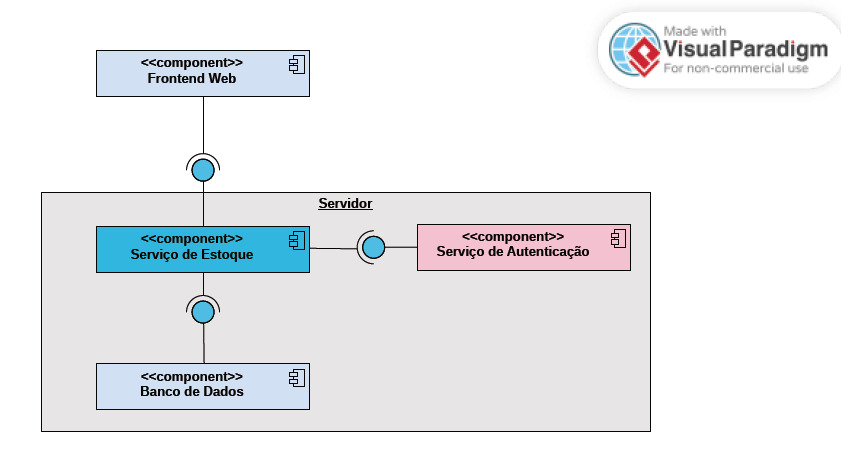
\includegraphics[width=1.0\textwidth]{Figuras/Componentes.png}


\subsubsection{Diagrama de Implantação}


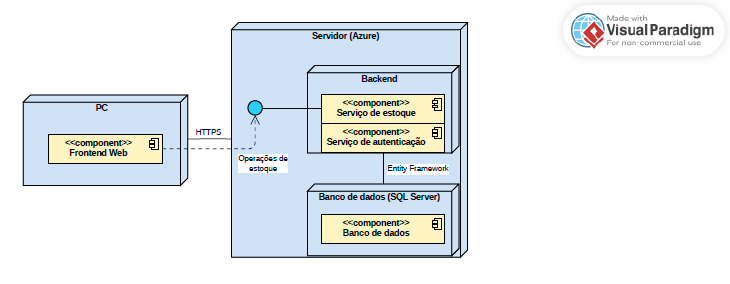
\includegraphics[width=1.0\textwidth]{Figuras/Implantação.png}



\section{Tecnologias}



\subsection{Front-end}


\subsection{Back-end}

\begin{itemize}
    \item \textbf{ASP.NET}: Framework desenvolvido pela Microsoft, utilizado para a criação de aplicações web robustas, seguras e escaláveis.
\end{itemize}

\subsection{Banco de Dados}

<<<<<<< Updated upstream
SQLServer ,
=======
\begin{itemize}
    \item \textbf{Microsoft SQL Server}: Banco de dados robusto e amplamente utilizado no mercado, responsável pelo armazenamento seguro das informações da aplicação.
\end{itemize}
>>>>>>> Stashed changes

\subsection{Infraestrutura}

\begin{itemize}
    \item \textbf{Microsoft Azure}: Plataforma de computação em nuvem utilizada para hospedar a aplicação e seus serviços relacionados. A utilização do Azure proporciona escalabilidade, segurança e alta disponibilidade.
\end{itemize}



\section{Testes de Manutenção}

\subsection{Plano de Testes}

\subsection{Análise Estatística}

\subsection{Testes Funcionais}

\subsection{Testes Não Funcionais}


\section{Segurança, Privacidade, Legislação}

Este tópico é dedicado a explicar sobre as questões de segurança e legislação relevantes para o noss projeto.

\subsection{Critérios de Segurança e Privacidade}

\subsection{Legislação}



\section{Modelo de Banco de Dados}


\subsection{MER}

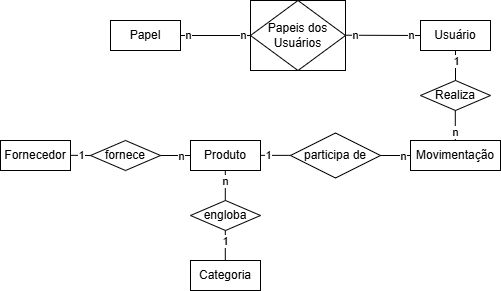
\includegraphics[width=1.0\textwidth]{Figuras/MERestoque.png}


\subsection{DER}

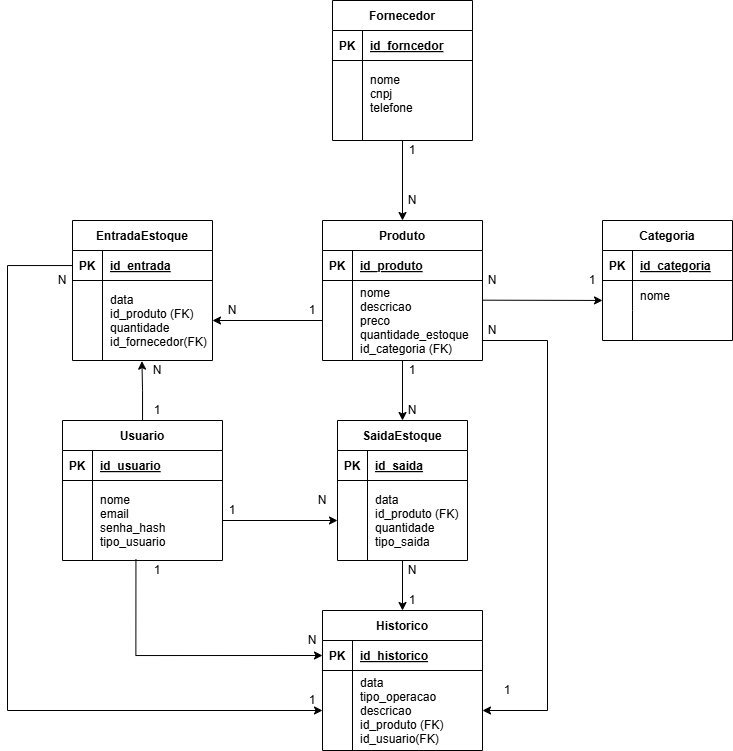
\includegraphics[width=1.0\textwidth]{Figuras/DERestoque.png}



\subsection{Dicionário de Dados}

\section{Cronograma}

\subsection{Análise da duração do projeto}

\chapter{Viabilidade Financeira}

\subsection{Custos}

\subsection{Receitas}

\subsection{Cenários}



\chapter{Considerações Finais}


\section{Dificuldades, escolhas}



% ---

\lipsum[24]

% ----------------------------------------------------------
% Finaliza a parte no bookmark do PDF
% para que se inicie o bookmark na raiz
% e adiciona espaço de parte no Sumário
% ----------------------------------------------------------
\phantompart




% ----------------------------------------------------------
% ELEMENTOS PÓS-TEXTUAIS
% ----------------------------------------------------------
\postextual
% ----------------------------------------------------------

% ----------------------------------------------------------
% Referências bibliográficas
% ----------------------------------------------------------
\bibliographystyle{abntex2-alf}
\bibliography{referencias}

% ----------------------------------------------------------
% Glossário
% ----------------------------------------------------------
%
% Consulte o manual da classe abntex2 para orientações sobre o glossário.
%
%\glossary

% ----------------------------------------------------------
% Apêndices
% ----------------------------------------------------------

% ---
% Inicia os apêndices
% ---
\begin{apendicesenv}

% Imprime uma página indicando o início dos apêndices
\partapendices

% ----------------------------------------------------------
\chapter{apendice exemplo}
% ----------------------------------------------------------

\lipsum[50]

% ----------------------------------------------------------
\chapter{Nullam elementum urna vel imperdiet sodales elit ipsum pharetra ligula
ac pretium ante justo a nulla curabitur tristique arcu eu metus}
% ----------------------------------------------------------
\lipsum[55-57]

\end{apendicesenv}
% ---


% ----------------------------------------------------------
% Anexos
% ----------------------------------------------------------

% ---
% Inicia os anexos
% ---
\begin{anexosenv}

% Imprime uma página indicando o início dos anexos
\partanexos

% ---
\chapter{exemplo 2}
% ---
\lipsum[30]

% ---
\chapter{Cras non urna sed feugiat cum sociis natoque penatibus et magnis dis
parturient montes nascetur ridiculus mus}
% ---

\lipsum[31]

% ---
\chapter{exemplo 3}
% ---

\lipsum[32]

\end{anexosenv}

%---------------------------------------------------------------------
% INDICE REMISSIVO
%---------------------------------------------------------------------
\phantompart
\printindex
%---------------------------------------------------------------------

\end{document}
